\chapter{Results}
\label{resultchapter}


%\section{Results}

%\begin{figure}[t]
%\begin{center}
%\setlength{\unitlength}{0.01\textwidth}
%\begin{picture}(100,30)
%\put(-5,-3.5){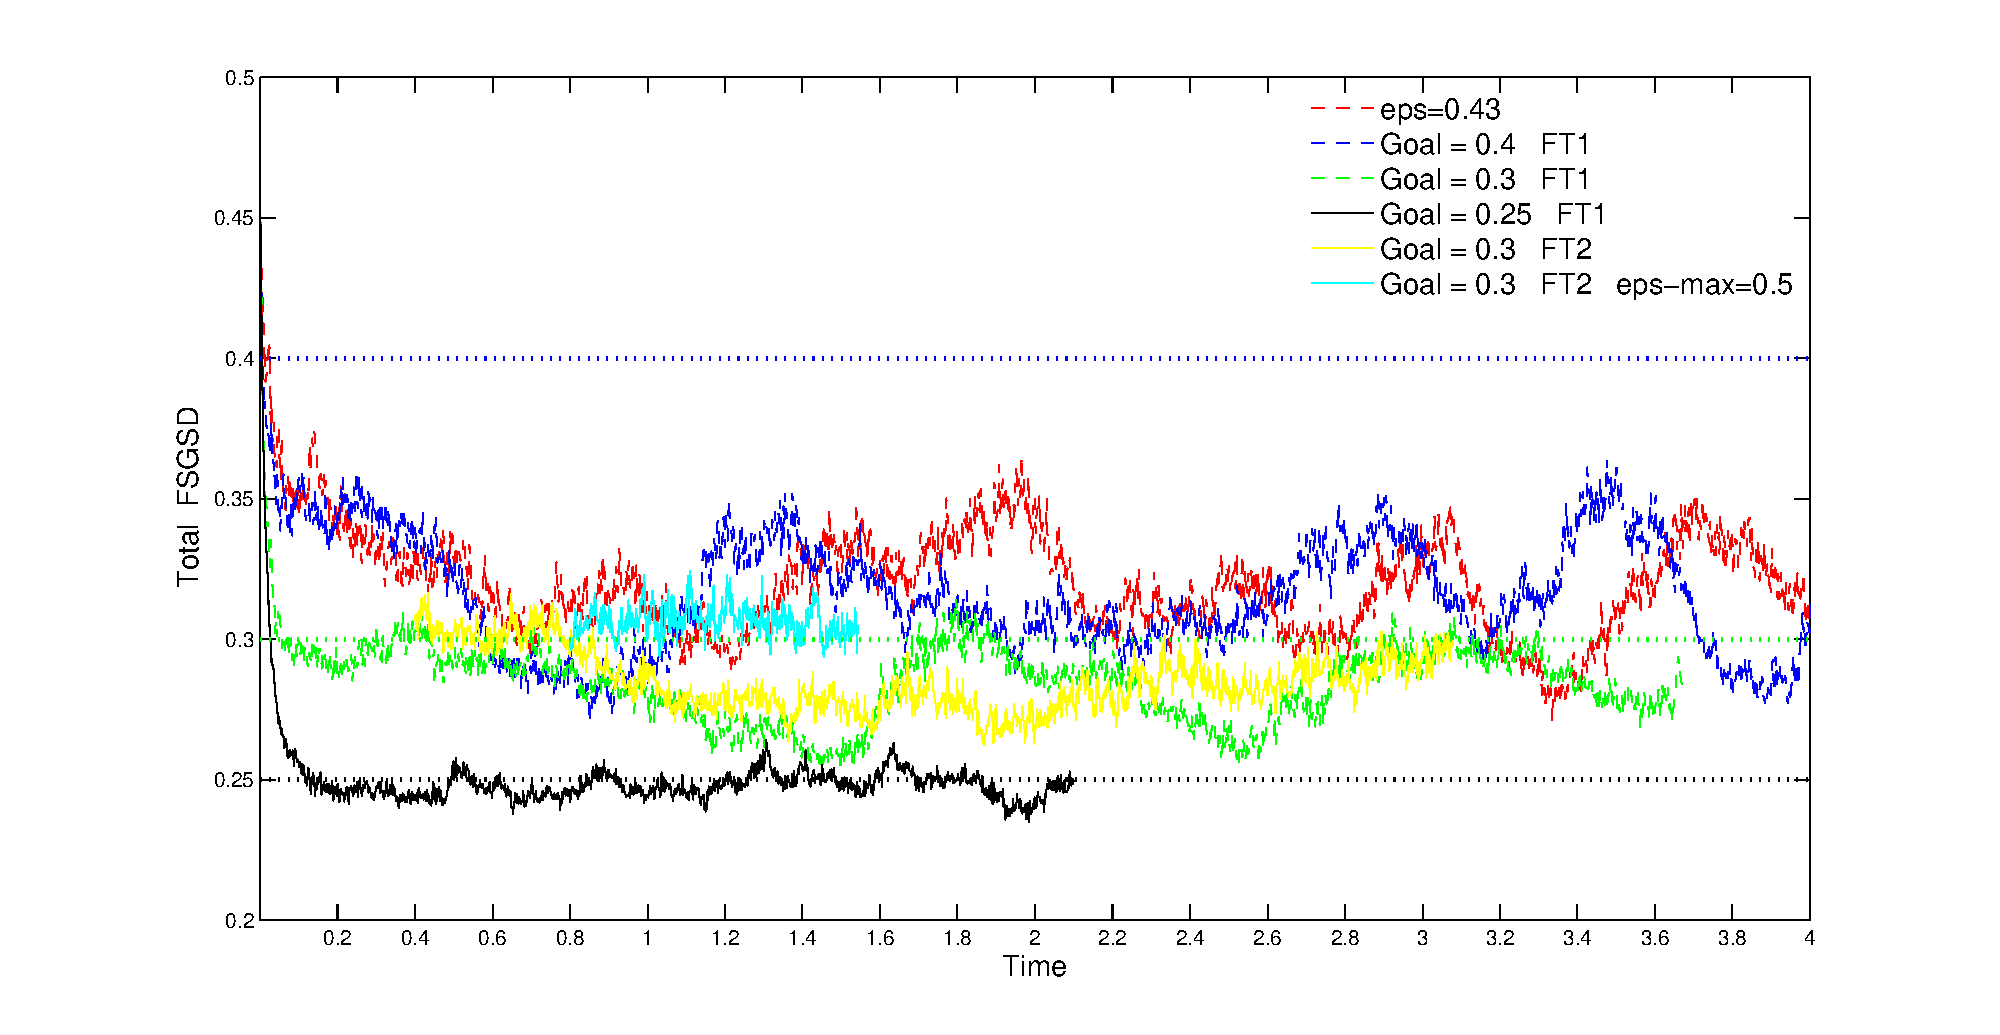
\includegraphics[height=0.34\textwidth]{figures/FSGSD_4.pdf}}
%\put(56,-3.5){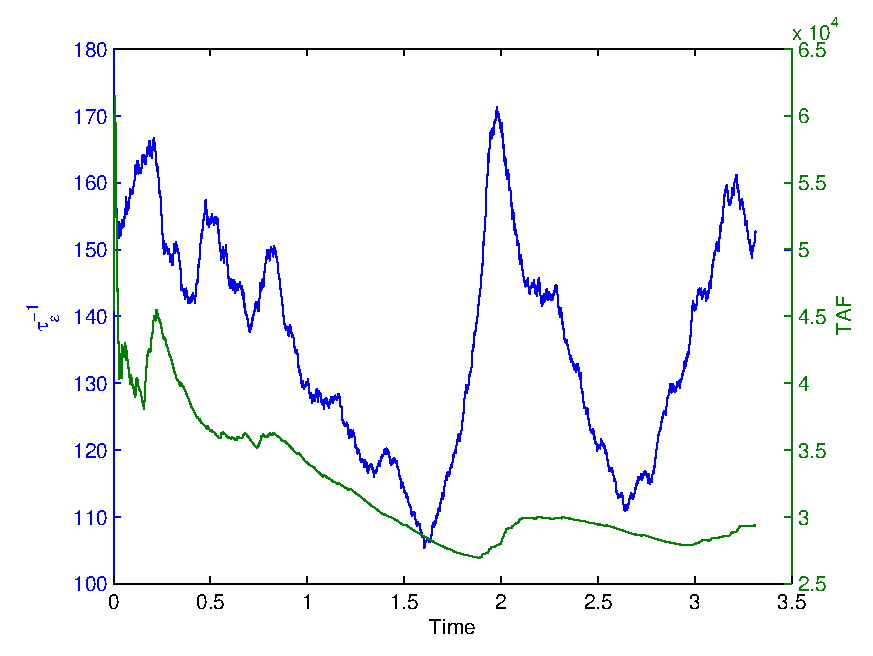
\includegraphics[height=0.34\textwidth]{figures/TAF__TauEps.pdf}}
%\put(4.5,25){(a)} \put(63,25){(b)}
%\end{picture}
%\end{center}
%\caption{Time-history of total fraction SGSD (a); Time-history of ${\rm TAF}$ and $\tau_{\epsilon}^{-1}$ (b). \vspace{-6pt}}
%\label{fig:FSGSD_FThistory}
%\end{figure}
%


\begin{figure}[t]
  \vspace{-10pt}
\begin{center}
  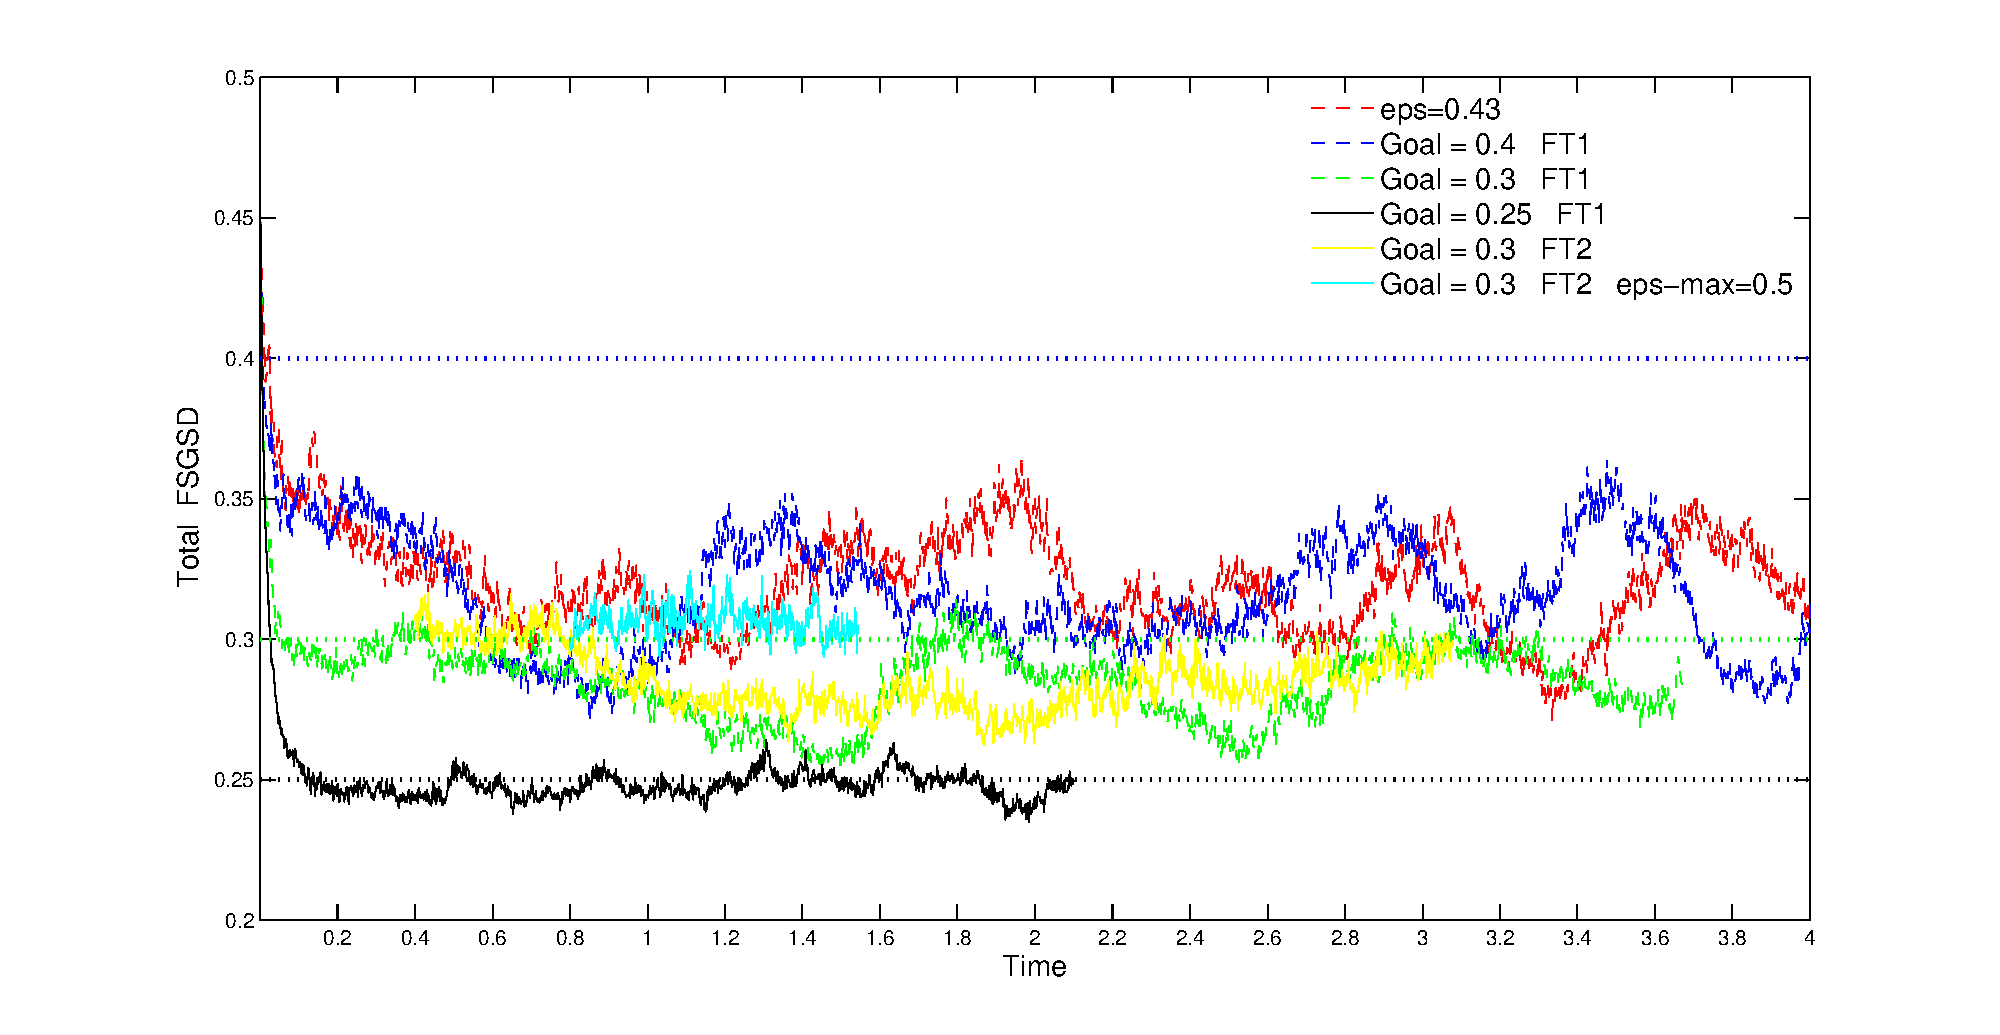
\includegraphics[width=0.9\textwidth]{figures/FSGSD_4.pdf}\\
\end{center}
  \vspace{-20pt}
  \caption{Time-history of total fraction SGSD.}
  \label{fig:FSGSD}
  \vspace{-10pt}
\end{figure}


The proposed methodology has been tested for linearly forced homogeneous turbulence \cite{JFM_2010}
with linear forcing constant coefficient $Q=6$
at $Re_{\lambda}\cong72$ (Taylor micro-scale Reynolds number)
using localized dynamic kinetic-energy-based SGS models \cite{POF_2008,JFM_2010}
on an adaptive grid with effective resolution $256^3$.
%The linear forcing constant coefficient, $Q$ was set to $6$.
%
Figure~\ref{fig:FSGSD} demonstrates the preliminary results of this implementation
for three different goal-values ($0.4, 0.3, 0.25$) for the local FSGSD with
the upper and lower bound for epsilon set as 0.2 and 0.43 ($\epsilon \in [0.2,0.43]$)
as well as a constant-thresholding case of  $\epsilon=0.43$ .
%
%of this technique to
The local and total FSGSD are defined respectively as
$
\frac{                            \Pi }
       {  \varepsilon_{\rm res}  +  \Pi }
$
and
%The Time-History of total fraction SGSD,
$
  \frac{                                         \langle \Pi \rangle }
       { \langle \varepsilon_{\rm res} \rangle + \langle \Pi \rangle }
$,
where
$\langle \Pi \rangle = \langle -\tau^*_{ij}
                                {{\left.\red\overline{\bl S}_{\bl ij} \rule{-8pt}{6pt}\right.}^{\red {\scriptscriptstyle >} \epsilon}}
                                %\bareps[S]_{ij}
                       \rangle$
and
$\langle \varepsilon_{\rm res} \rangle = 2 \nu \langle
                                                {{\left.\red\overline{\bl S}_{\bl ij} \rule{-8pt}{6pt}\right.}^{\red {\scriptscriptstyle >} \epsilon}}
                                                {{\left.\red\overline{\bl S}_{\bl ij} \rule{-8pt}{6pt}\right.}^{\red {\scriptscriptstyle >} \epsilon}}
                                                %\bareps[S]_{ij} \bareps[S]_{ij}
                                               \rangle$
are respectively  the volume-averaged SGS dissipation and the volume-averaged resolved viscous dissipation .


%where $\varepsilon_{\rm res}$ is resolved viscous dissipation.
%
For the case of Goal=0.4, total-FSGSD never reaches the prescribed goal-value ($0.4$).
The reason is that the total-FSGSD for the case of constant-thresholding with $\epsilon=0.43$ is than $0.4$ for most of the time.
As a result, varying thresholding-factor with a ``local-FSGSD goal-value'' larger than the average FSGSD of constant-thresholding
using the same $\epsilon$ and $\epsilon_{\max}$ resulted in total-FSGSD, which was bellow the goal-value.
Similarly to the previous case, the test case of the goal-value of 0.3 inherits a large-period oscillations due to capping $\epsilon$ at $0.43$ level regardless of the forcing method.
These oscillations are removed by increasing $\epsilon_{\max}$ to $0.5$.
The success of this test with larger $\epsilon_{\max}$ compared with the above mentioned two tests,
where $\epsilon_{\max}$ was $0.43$,
revealed that the upper bound of the interval for allowable threshold variations
was not large enough to increase the SGS dissipation accordingly,
which implies that with $\epsilon \in [0.2,0.43]$ flow was over resolved.
Therefore, to achieve a FSGSD greater than the average of FSGSD corresponding to constant-thresholding at a certain $\epsilon_{\rm constant-thresholding}$,
it is required to set the  $\epsilon_{\max} > \epsilon_{\rm constant-thresholding}$.
This is further confirmed by considering the case with  the goal set to $0.25$, which illustrates  how precisely the spatially variable thresholding methodology can
maintain $\Pi$ at a priori defined level. In addition, when $\epsilon_{\max}$ is set up high enough,  the  SGS dissipation approaches the desired level within
few eddy turnover times.

%\noindent
%The time history of $400 \, {\rm TAF}^{-1}$ and $\tau_{\epsilon}^{-1}$ are shown in Figure ~\ref{fig:FThistory}.
The time history of ${\rm TAF}$ and $\tau_{\epsilon}^{-1}$ are shown in Fig.~\ref{fig:FThistory}.
The relaxation time parameter for FT2, $\tau_{\epsilon}$, is approximately one-tenth of
the large eddy turnover time,
$\tau_{\rm eddy}= \frac{u'^2}{\langle \varepsilon \rangle} = \frac{ \frac 2 3 K}{2 K Q} = \frac 1 {3Q}= \frac 1 {18}$.
While the relaxation time parameter for FT1, $C_{{\rm f}_{\epsilon}} {\rm TAF}^{-1}$, is between one-third and one-fourth of $\tau_{\rm eddy}$.
That is, FT2 has as much as 2 to 3 times faster response compared with FT1.
%In fact, the intentional choice of $400$ factor in FT1 was to make make FT1 response about three to four times faster than $\tau_{\rm eddy}$
%which is much slower thatn the response of FT2 ($\sim 10 \tau_{\rm eddy}$).
This faster time response was able to partially recover the FSGSD.
This improvement reveals the importance of very localized and fast mechanisms for the forcing term.
%
The time-averaged term in FT1 destroys the localized Lagrangian nature of the algorithm;
however, to smear out the effect of possible very localized FSGSD values, it is recommended to have some averaging mechanism.
Hence, another approach, which is currently under investigation,
is to track the forcing term itself within a Lagrangian frame so that
the forcing term inherits the history of the flow evolution.



\begin{figure}[t]
  \vspace{-20pt}
\begin{center}
  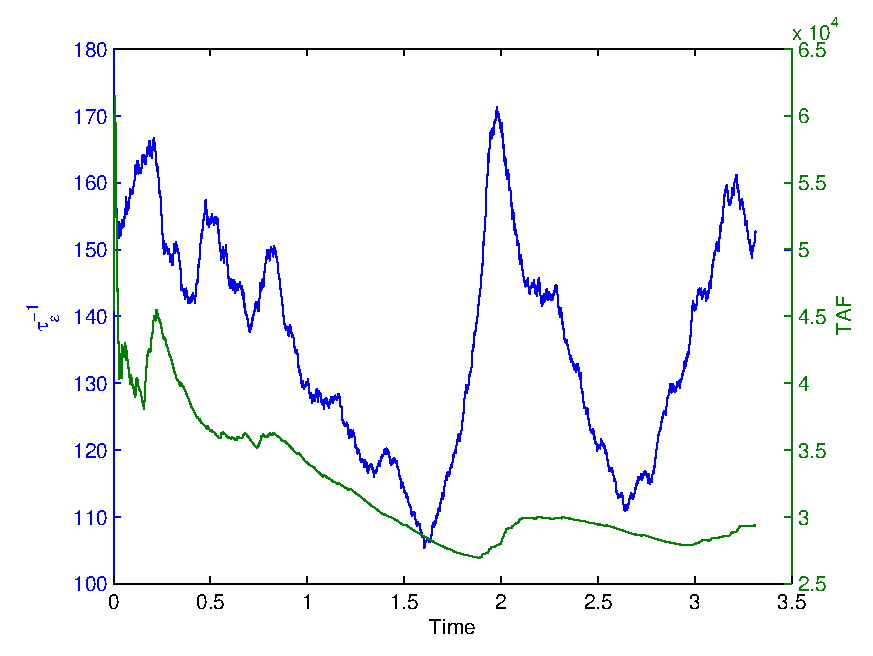
\includegraphics[width=0.7\textwidth]{figures/TAF__TauEps.pdf}\\
\end{center}
  \vspace{-20pt}
  \caption{Time-history of ${\rm TAF}$ and $\tau_{\epsilon}^{-1}$.}
  \label{fig:FThistory}
%\vspace{-20pt}

  \vspace{-20pt}
\begin{equation}
 \nonumber
%\setlength{\extrarowheight}{0.3cm}
\begin{array}{lrcrl}

\vspace*{.2cm}

{\rm Relaxation \; Time \; Parameter \; for \; FT1:} \;\; &
C_{{\rm f}_{\epsilon}} \, {\rm TAF}^{-1} &
\;\;\;
\approx
\;\;\;&
\frac 1 {3 \, {\rm or} \, 4}&
\tau_{\rm eddy} \;\;\; (\frac 1 {75})\\ %= \frac 1 {3Q}= \frac 1 {18}

%\vspace*{0.2cm}

{\rm Relaxation \; Time \; Parameter \; for \; FT2:} \;\;&
\tau_{\epsilon}&
\;\;\;
\approx
\;\;\;&
\frac 1 {10}&
\tau_{\rm eddy} \;\;\; (\frac 1 {170})  %= \frac 1 {3Q}= \frac 1 {18}

\end{array}
\end{equation}
  \vspace{-12pt}

\end{figure}




Analysis of spatially variable thresholding SCALES by means of the localized dynamic kinetic-energy model (LDKM)
-- in which either Bardina-like or Germano-like approach is exploited for the dynamical evaluation of both
turbulent eddy-viscosity and SGS energy dissipation model coefficients --
to close the filtered momentum equations
is the subject of further investigations.


Time history of number of active wavelets, ${\rm Nwlt}$, shows that for small goal value  of 0.25,
number of grid points by average is higher while all the other variable thresholding cases inherit approximately the
same average of number of active wavelets compared with the constant-threshold case of $\epsilon=0.43$, Fig.~\ref{fig:nwlt}.

Compression Ratio, ${\rm Nwlt / Nwlt_{Max}}$ --
which is the ratio of the active wavelets on the adaptive grid to
the total available wavelets on the non-adaptive effective grid at the highest level of resolution or DNS resolution of $256^3$ --
illustrated a compression of less than 1\% at most of the time for all cases except Goal=$0.25$, Fig.~\ref{fig:nwltNwlt}. Even for Goal=$0.25$, the compression is retained at less than 2 \%. Considering that the sixth order AWCM code is about 3 to 5 times slower per grid point than pseudo-spectral DNS code \cite{JFM_2010},
%the compression factor of even 2\% at the worst case scenario,
even the worst case scenario of compression factor of 2\%,
represents an acceleration of approximately 16 to 10 times with
respect to pseudo-spectral DNS. This clarifies the enormous compression, i.e. number one strength of the wavelets in turbulence.

%... yet less than \%2 of non-adaptive grid, at the highest level of resolution, or DNS grid ...
%again, the compression -- number one beauty of the wavelets in turbulence -- is evident at ...
%though adaptive schemes are not cheap but in parallel with a scalable code, the adaptive scheme cost is acceptable, i.e.
%it is not ignorable but it is affordable.

Total Resolved Dissipation, $\langle \varepsilon_{\rm res} \rangle$, Fig.~\ref{fig:RD}, indicates that not necessarily the smaller goal value for FSGSD results in higher resolved dissipation at all time. This is becasue of the fact that the continuous coupling between the dissipation and grid-adaptation results in continuous adjustment of resolved dissipation as discussed before by refining or coarsening the grid and as a result at some time/locations it may affect the amplitude of the resolved dissipation differently. Therefore, one can not make such a judgement whether the lower FSGSD goal value means the the higher resolved dissipation throughout the spatial/time space. This argument is valid for the
Total SGS Dissipation,  $\langle \Pi \rangle$, and
Total Resolved+SGS Dissipation, $\langle \varepsilon_{\rm res} \rangle + \langle \Pi \rangle$,
as illustrated in Figures ~\ref{fig:SGSD} and ~\ref{fig:TotalD} respectively.

Taylor Microscale Reynolds Number, $Re_{\lambda}= \frac {u'\lambda} {\nu}$,
where the Taylor length-scale can be evaluated for isotropic turbulence as
$\lambda = (\frac {15 \nu u'^2}  {\langle \varepsilon \rangle})^{1/2}$,
is demonstrated in Fig.~\ref{fig:ReTaylor} where the time averaged of each case is also shown.


\clearpage 
\newpage

\begin{figure}[t]
  \vspace{-20pt}
\begin{center}
  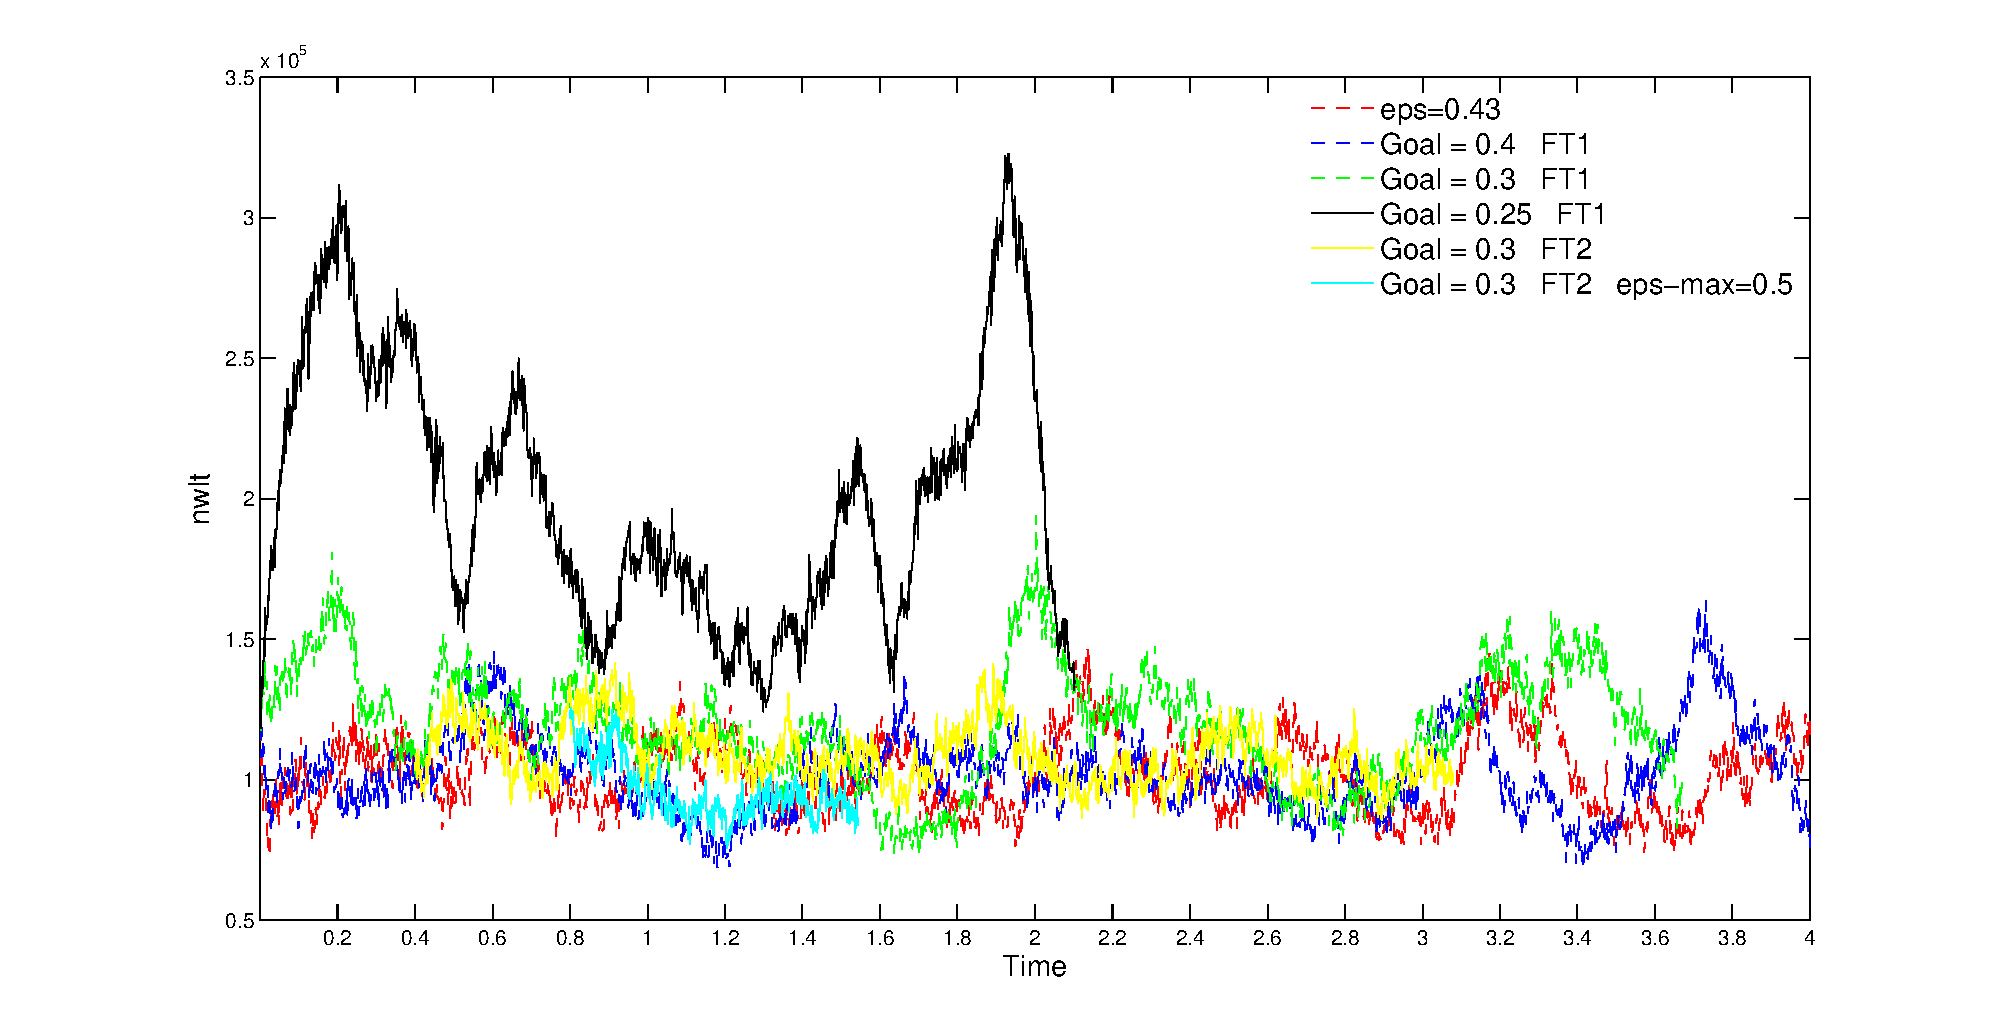
\includegraphics[width=0.9\textwidth]{figures/Statistics/nwlt.pdf}\\
\end{center}
  \vspace{-20pt}
  \caption{Number of Active Wavelets.}
  \label{fig:nwlt}
\end{figure}



\begin{figure}
  \vspace{-20pt}
\begin{center}
  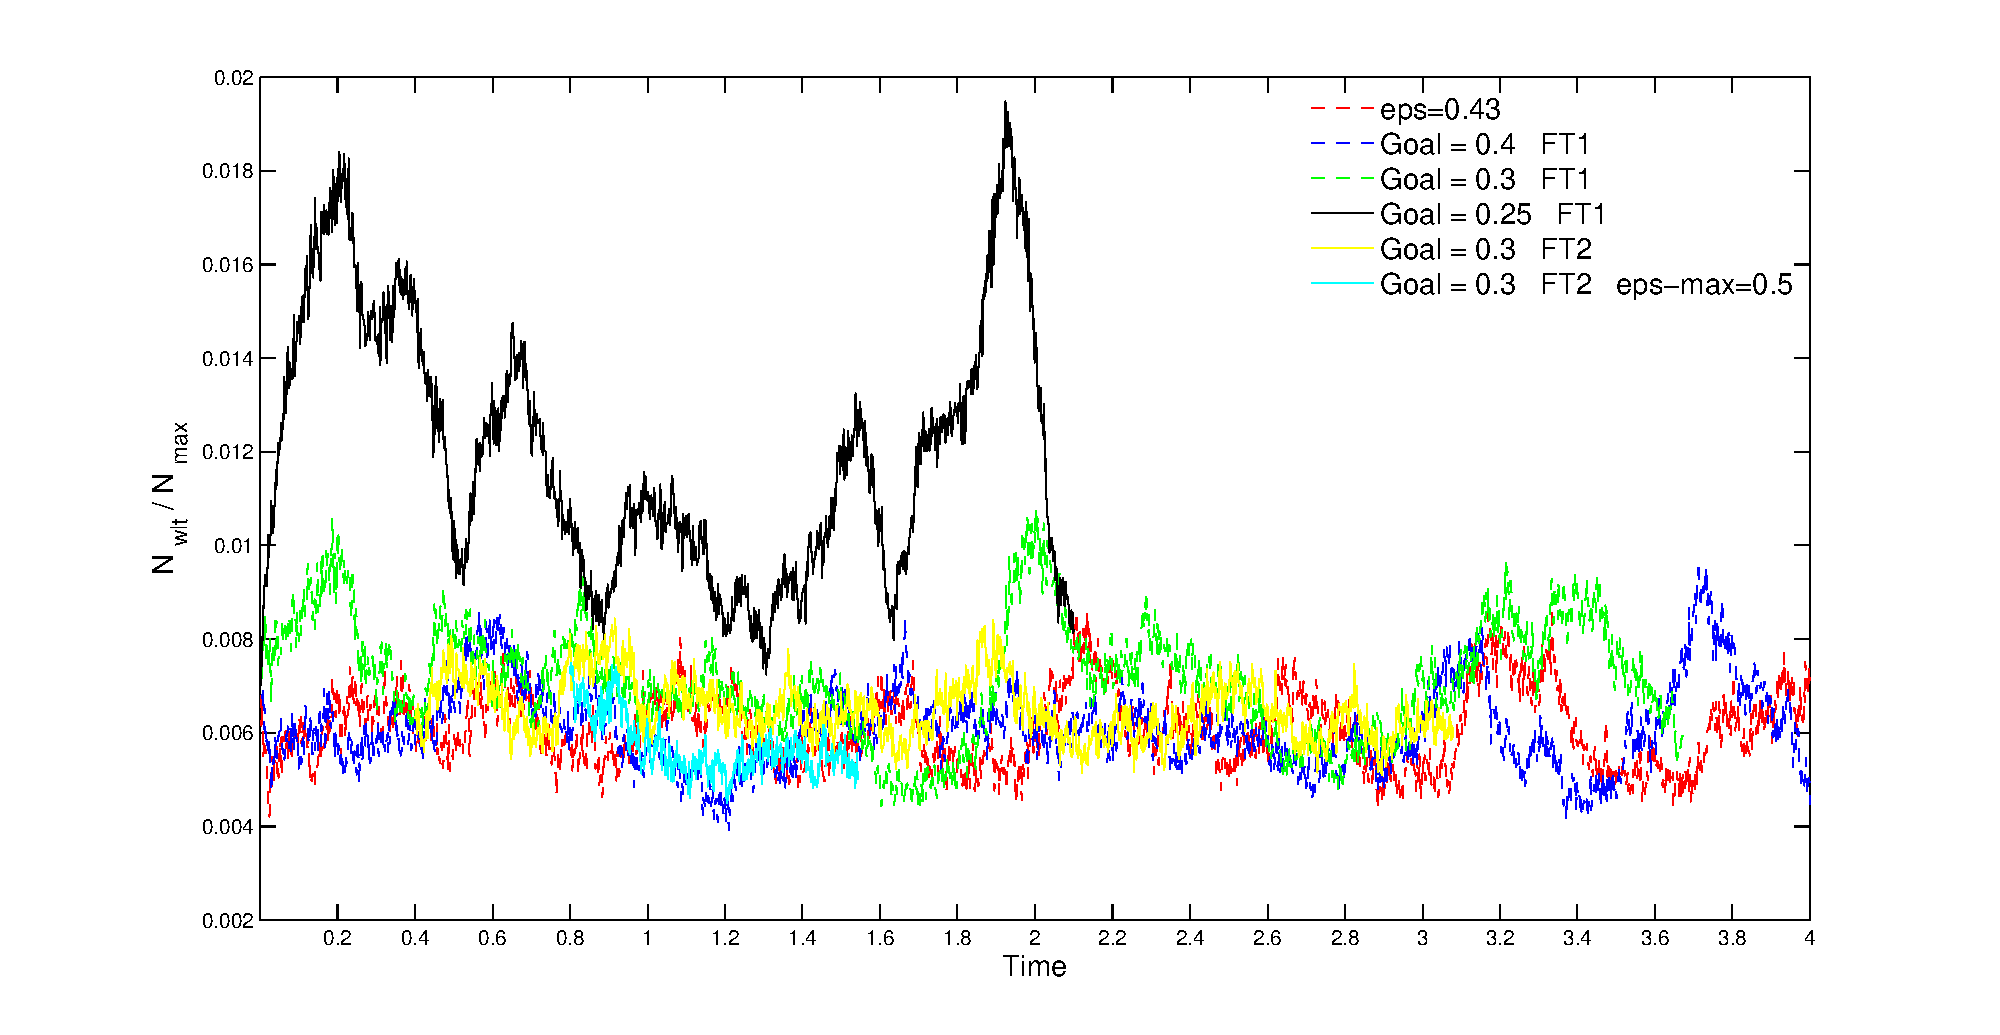
\includegraphics[width=0.9\textwidth]{figures/Statistics/Nwlt_Nmax.pdf}\\
\end{center}
  \vspace{-20pt}
  \caption{Compression Ratio.}
  \label{fig:nwltNwlt}
\end{figure}



\begin{figure}
  \vspace{-20pt}
\begin{center}
  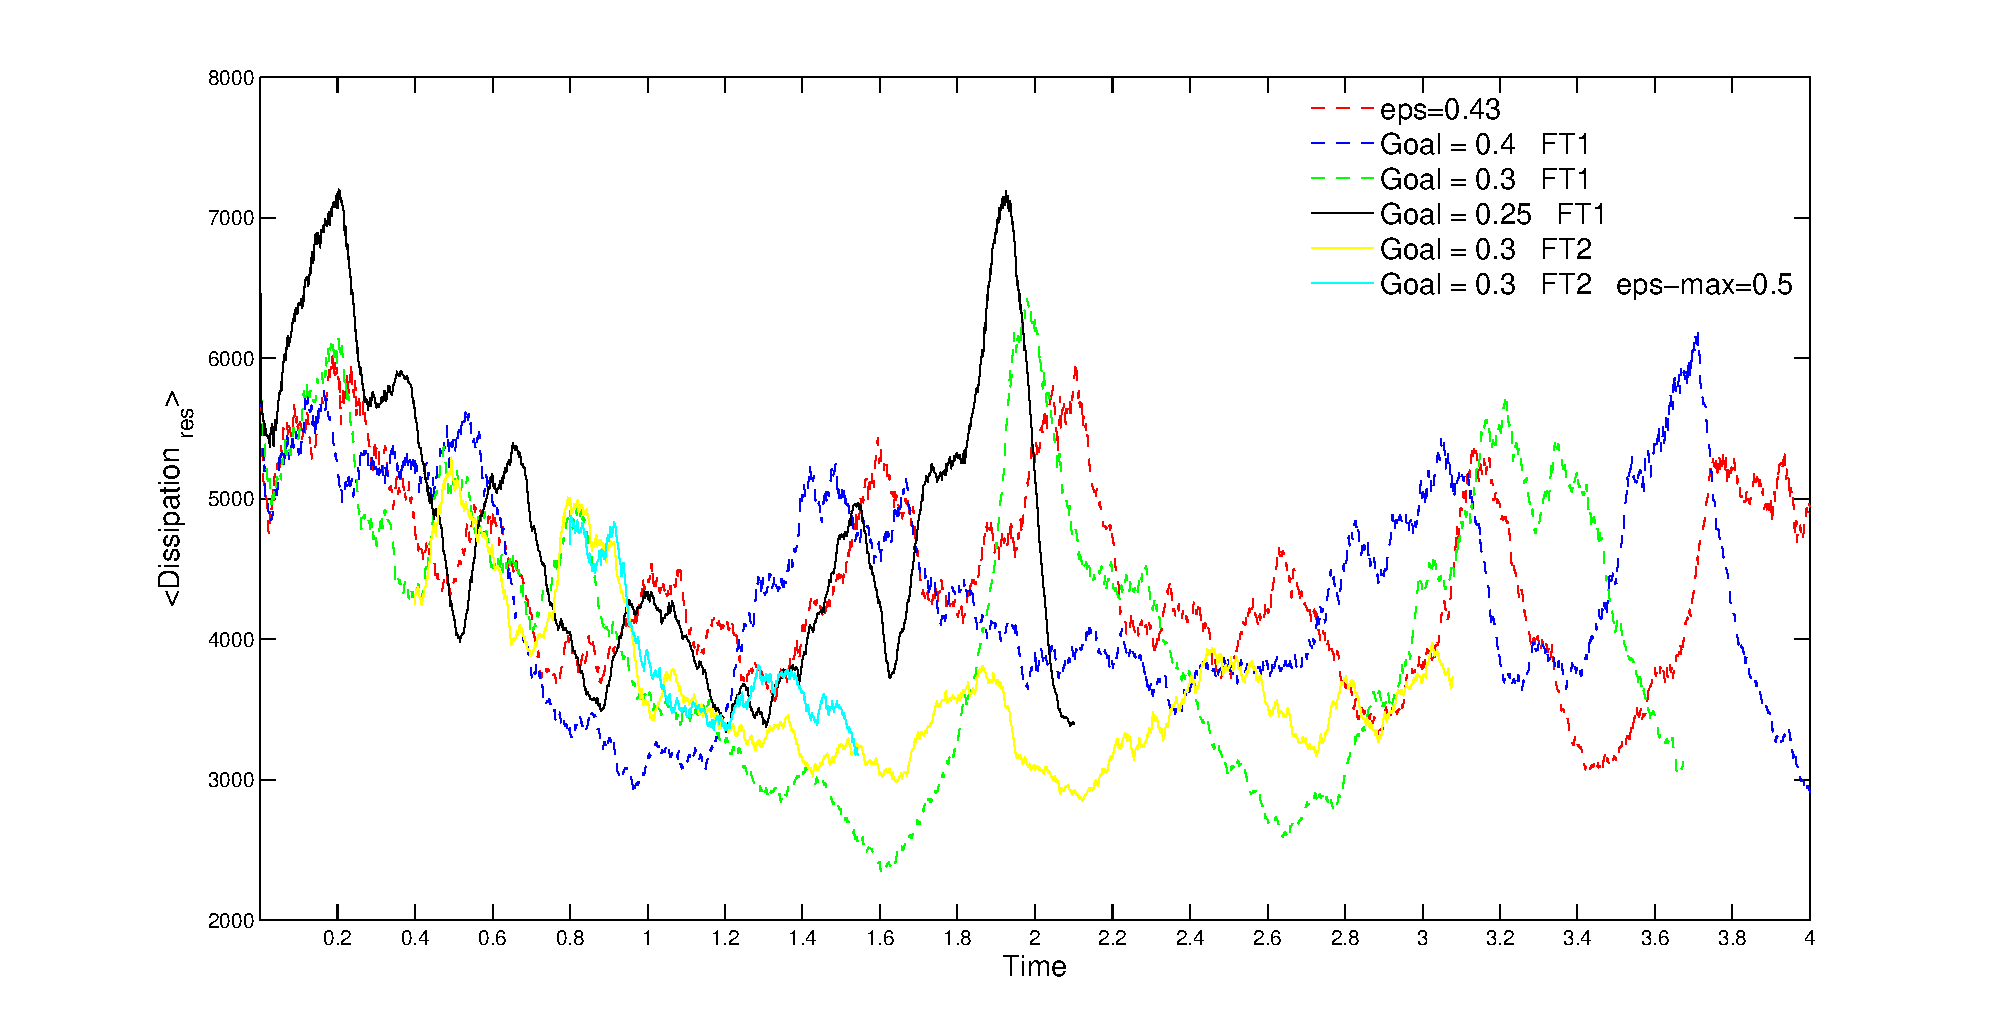
\includegraphics[width=0.9\textwidth]{figures/Statistics/TotalResolvedDissipation.pdf}\\
\end{center}
  \vspace{-20pt}
  \caption{Total Resolved Dissipation, $\langle \varepsilon_{\rm res} \rangle$.}
  \label{fig:RD}
\end{figure}


\clearpage
\newpage


\begin{figure}[t]
  \vspace{-20pt}
\begin{center}
  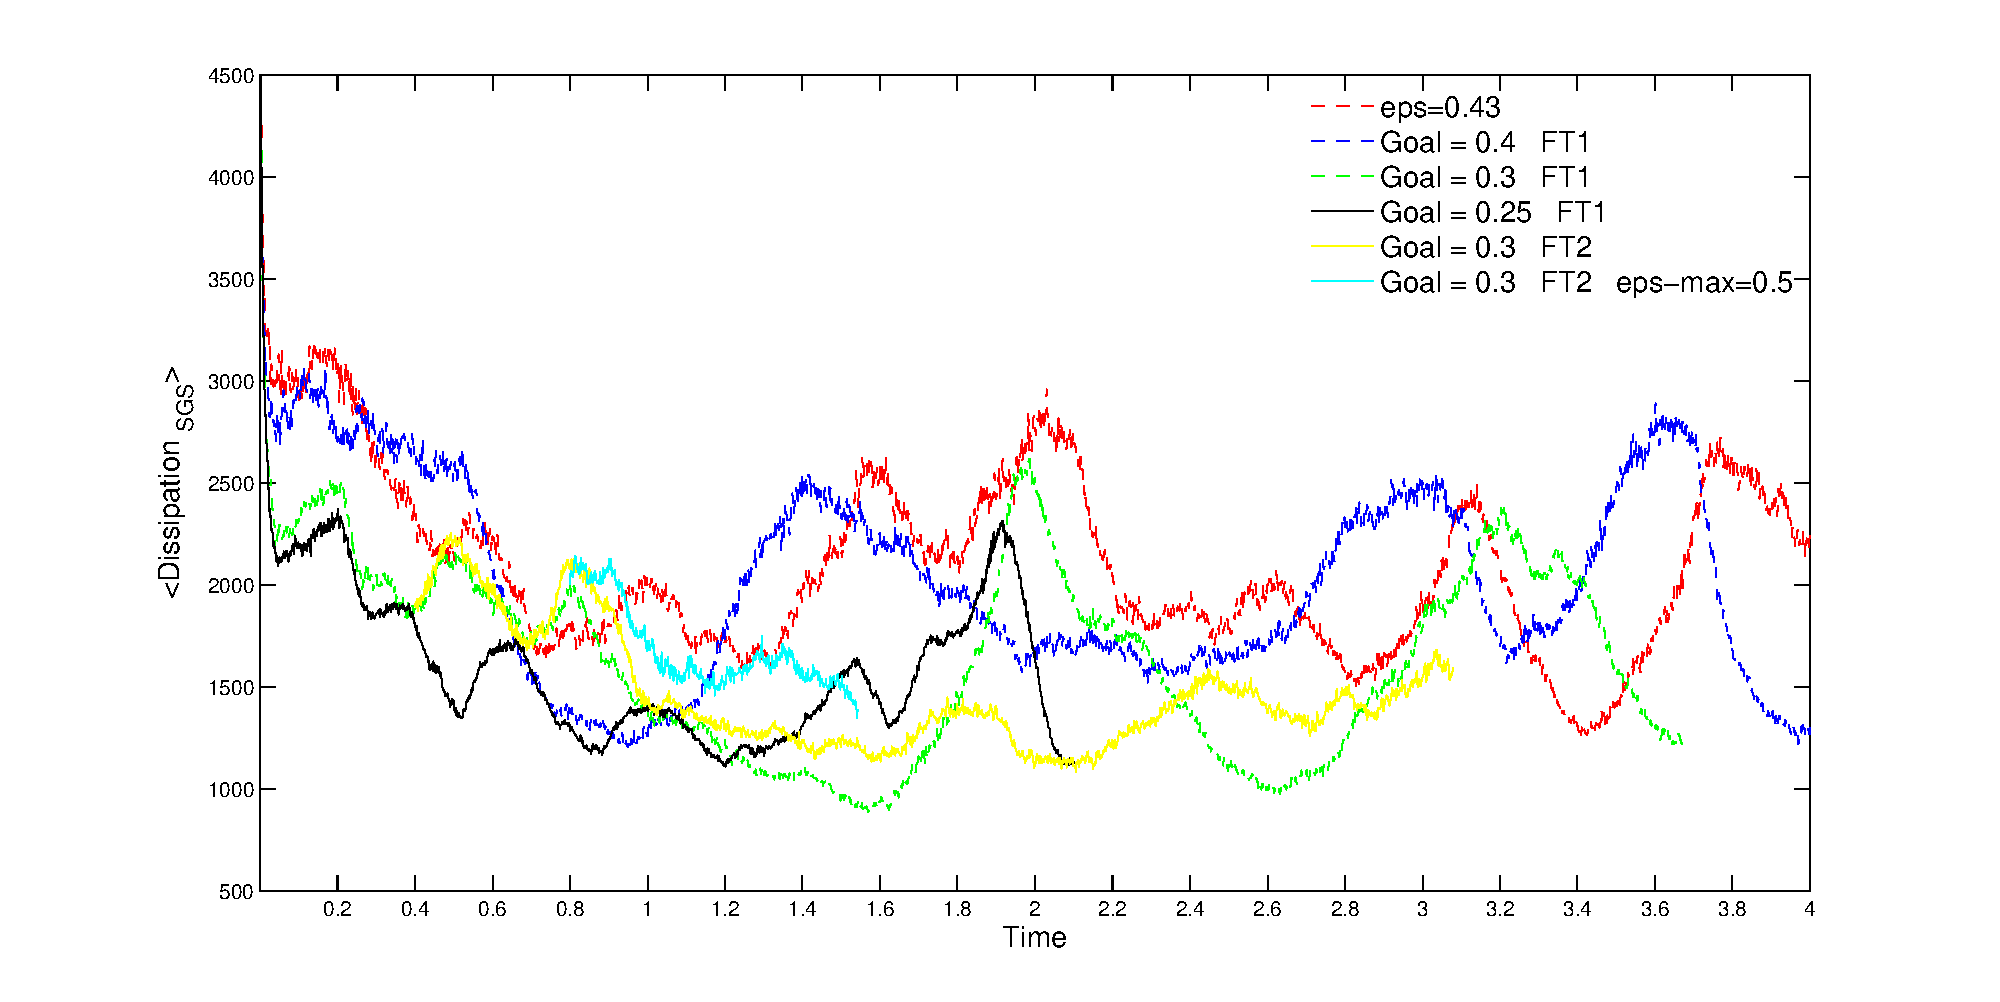
\includegraphics[width=0.9\textwidth]{figures/Statistics/TotalSGSDissipation.pdf}\\
\end{center}
  \vspace{-20pt}
  \caption{Total SGS Dissipation,  $\langle \Pi \rangle$.}
  \label{fig:SGSD}
\end{figure}



\begin{figure}
  \vspace{-20pt}
\begin{center}
  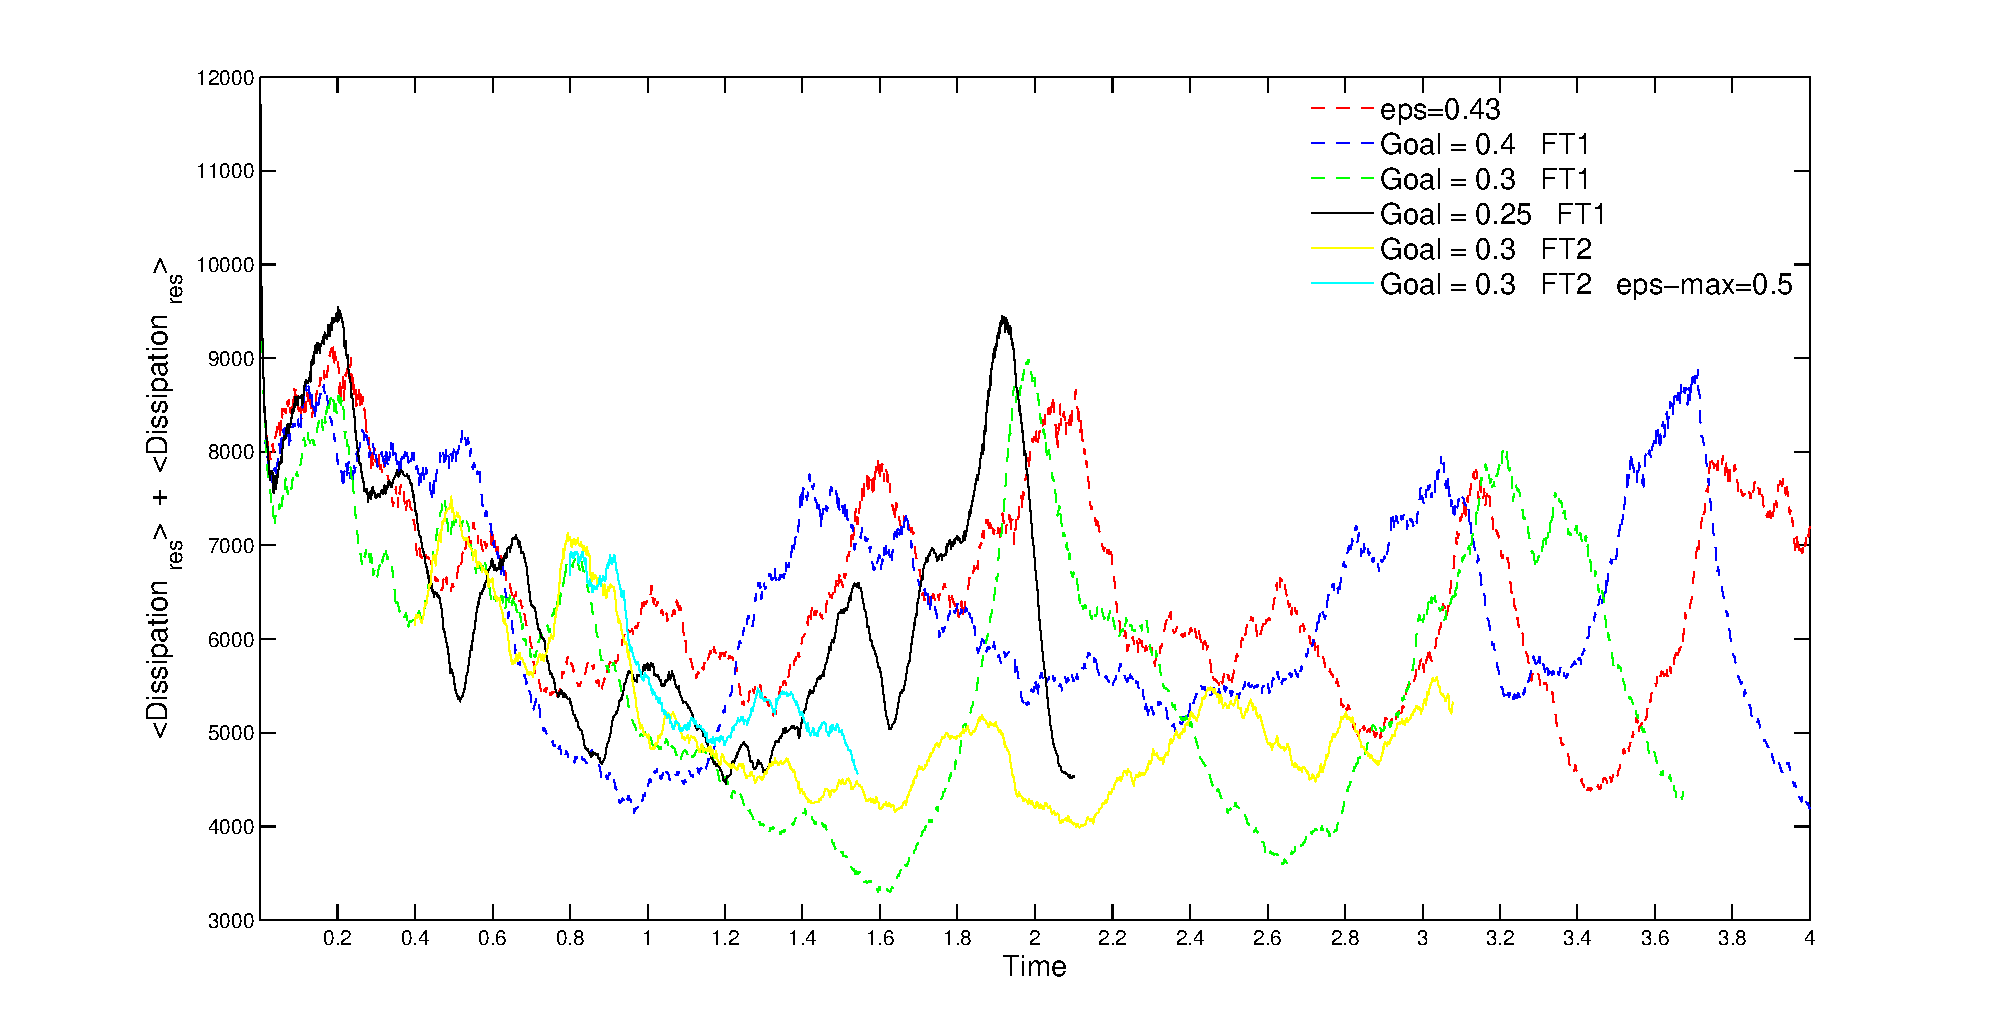
\includegraphics[width=0.9\textwidth]{figures/Statistics/TotalResolved+SGSDissipation.pdf}\\
\end{center}
  \vspace{-20pt}
  \caption{Total Resolved+SGS Dissipation, $\langle \varepsilon_{\rm res} \rangle + \langle \Pi \rangle$.}
  \label{fig:TotalD}
\end{figure}



\begin{figure}
  \vspace{-20pt}
\begin{center}
  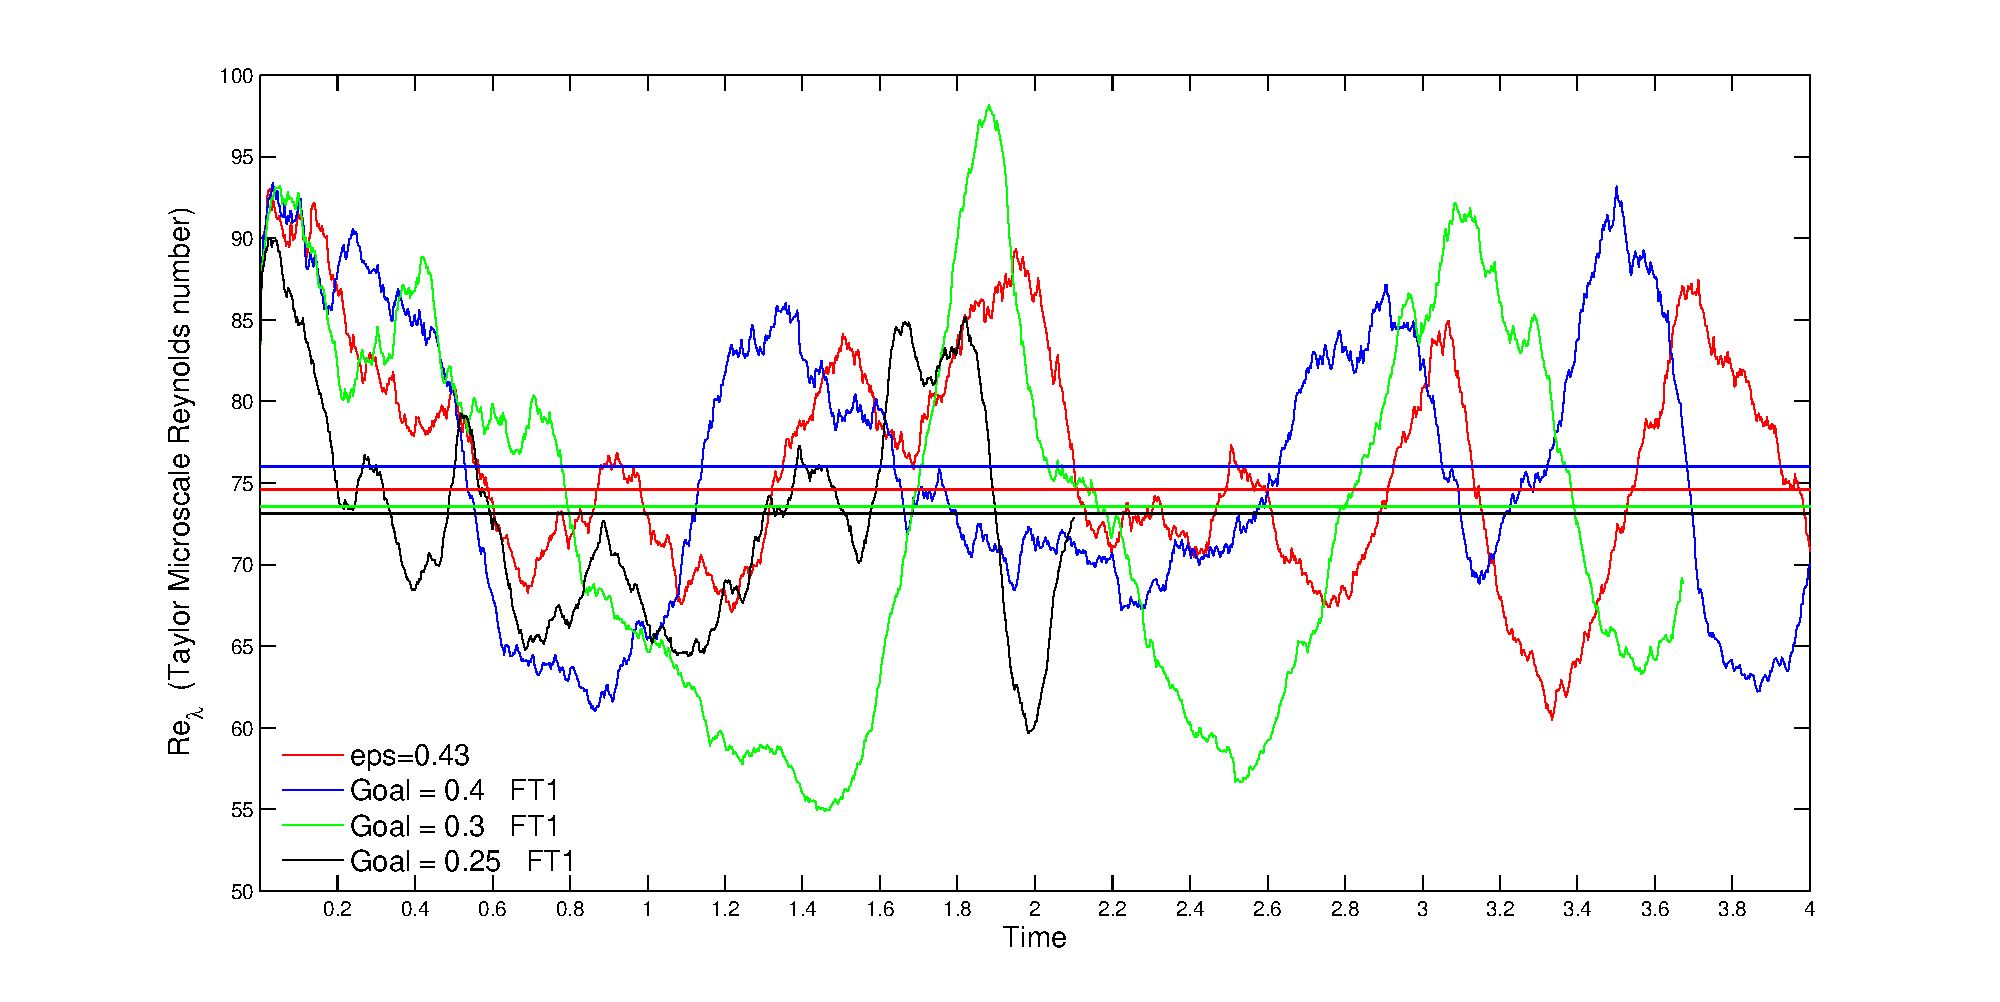
\includegraphics[width=0.9\textwidth]{figures/Statistics/ReTaylor.pdf}\\
\end{center}
  \vspace{-20pt}
  \caption{Taylor Microscale Reynolds Number, $Re_{\lambda}$.}
  \label{fig:ReTaylor}
\end{figure}












%\begin{figure}[t]
%\centerline{
%%\includegraphics[width=8cm, clip=true, viewport=2.3cm 1cm 32cm 17cm]{figures/FSGSD.pdf}}   %0cm 0cm 40cm 40cm
%\includegraphics[width=4cm]{figures/FSGSD_1_RGB.pdf}}
%\caption{Time-history of total fraction SGSD.}
%\label{fig:FSGSD}
%\end{figure}
%
%\begin{figure}[t]
%%\sidecaption[t]
%%\centerline{
%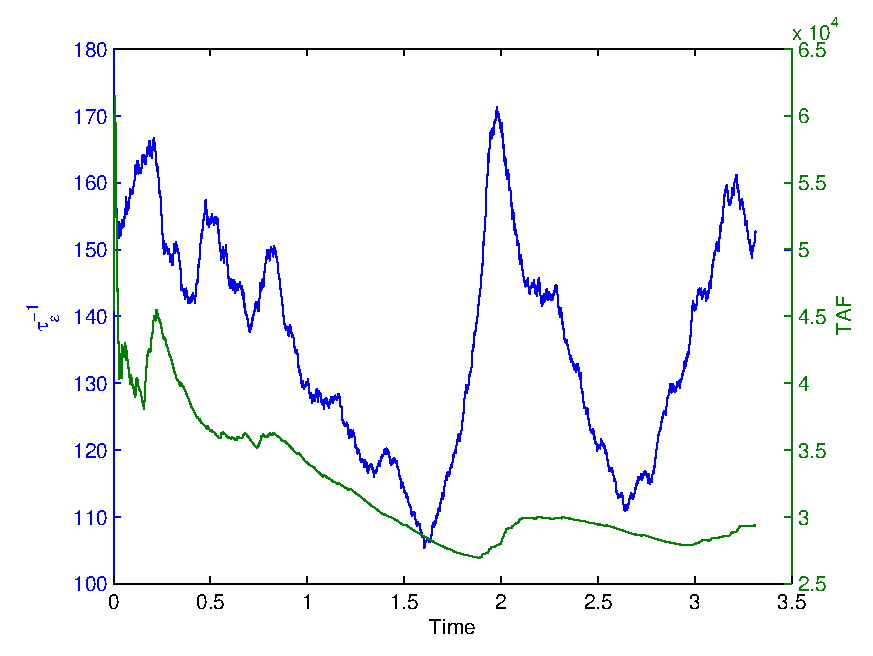
\includegraphics[width=4cm]{figures/TAF__TauEps.pdf}
%%}
%\caption{Time-history of \newline ${\rm TAF}$ and $\tau_{\epsilon}^{-1}$.}       %$400 \, {\rm TAF}^{-1}$
%\label{fig:FThistory}
%\end{figure}










%\section{Perspective}
%
%To summarize, variable thresholding is a methodology, which provides two-way feedback between the modeled SGS dissipation and the computational mesh
%in order to maintain a priori defined level of SGS dissipation, namely a prescribed level of turbulence resolution.
%The feedback is achieved through spatio-temporal variation of the wavelet threshold  that follows the evolution of the resolved/unresolved flow structures. The proposed methodology represents a \emph{fully adaptive wavelet thresholding filter} for turbulent flow simulation, where the thresholding level  is determined on the fly by tracking the areas of locally significant
%SGS dissipation (or any other physical quantity).
%
%Finally, in words of Marcel Lesieur \cite{Book_Turbulence_Lesieur},
%\begin{quotation}
%It might finally happen that this would be only a necessary transition stage toward the definition of new fluid dynamical concepts
%which would render obsolete and useless the complicated analytical and numerical techniques which helped create them.
%\end{quotation}


\clearpage
\newpage


To summarize, variable thresholding is a methodology, which provides two-way feedback between the modeled SGS dissipation and the computational mesh
in order to maintain a priori defined level of SGS dissipation, namely a prescribed level of turbulence resolution.
The feedback is achieved through spatio-temporal variation of the wavelet threshold  that follows the evolution of the resolved/unresolved flow structures. The proposed methodology represents a \emph{fully adaptive wavelet thresholding filter} for turbulent flow simulation, where the thresholding level  is determined on the fly by tracking the areas of locally significant
SGS dissipation (or any other physical quantity).


This methodology has been also tested for external flow applications where forcing term of ``characteristic based tracking of epsilon'' is
constructed based on the magnitude of vorticity or strain rate.
The results for incompressible flow around NACA 0015 airfoil show a
very robust and fast methodology for adjusting the thresholding-factor based on dynamically
important flow characteristics, for instance, the magnitude of vorticity or strain rate (Figure ~\ref{fig:NACA0015}).

\begin{figure}[htp]
  \vspace{-20pt}
\begin{center}
  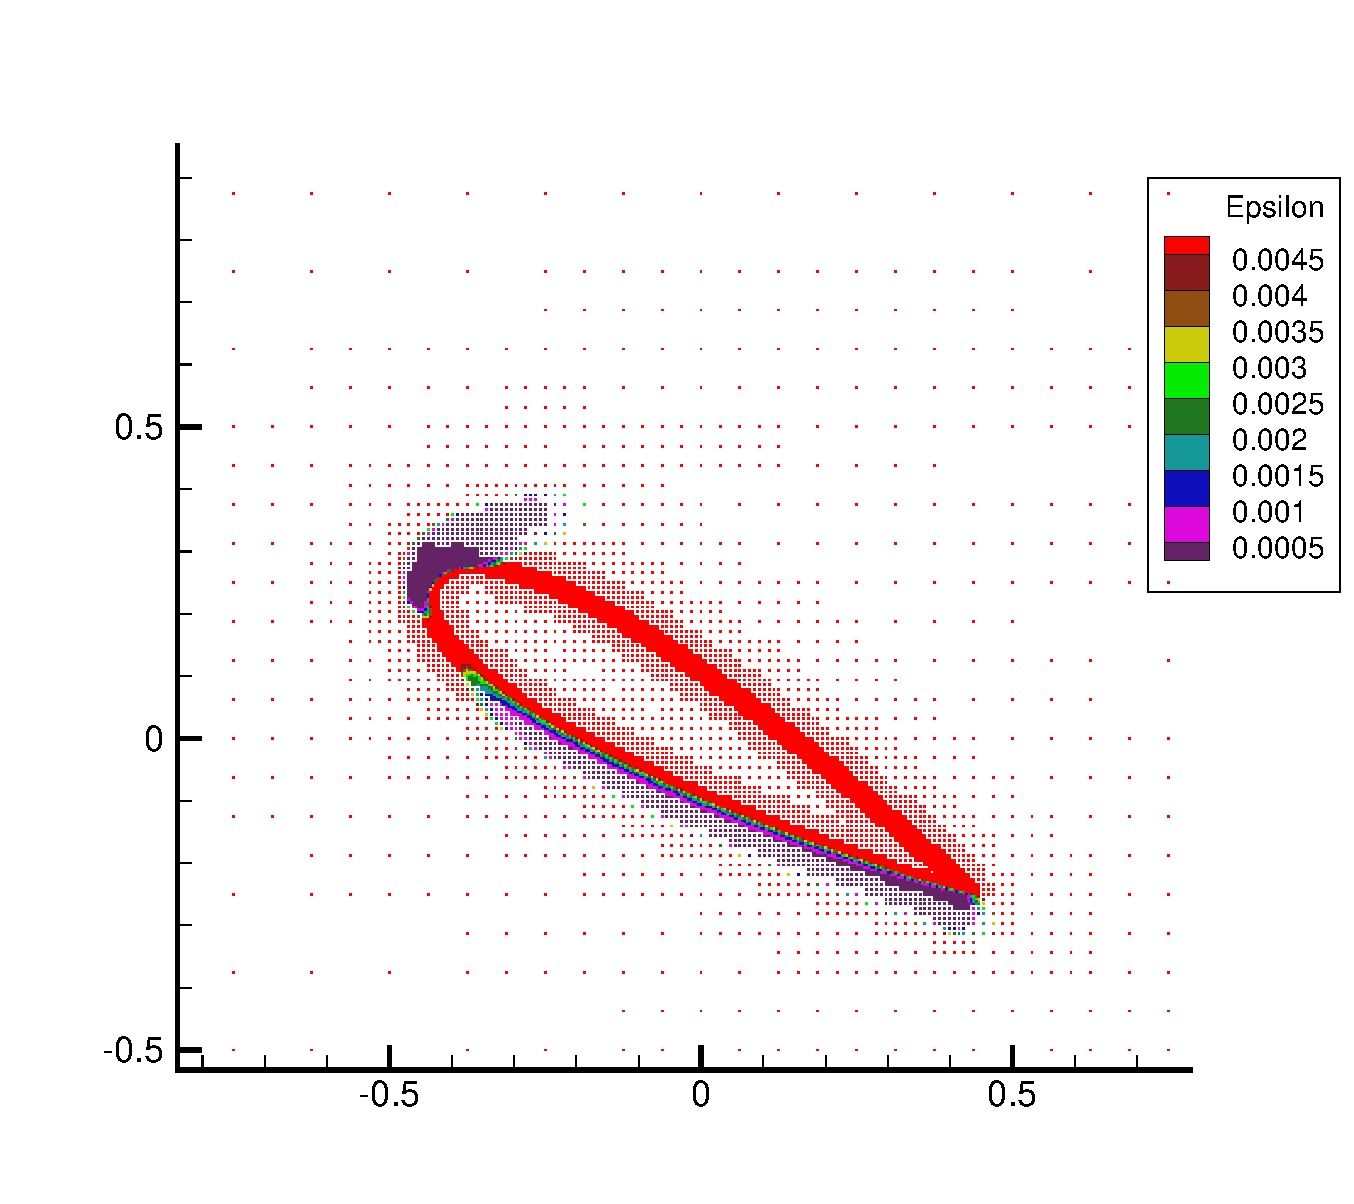
\includegraphics[width=0.8\textwidth]{figures/NACA0015.pdf}
\end{center}
  \vspace{-30pt}
  \caption{Incompressible flow around NACA 0015 at $30\,^{\circ}$ angle-of-attack.}
  \label{fig:NACA0015}
\end{figure}

